%!TEX encoding = UTF-8 Unicode
%!TEX root = ../thesisCASes.tex

%% TITOLO
\section{Sistemi Caotici}
\label{sec:Sistemi Caotici}

Ciò che accomuna un sistema complesso ad un sistema caotico è la non linearità.
In questa visione della complessità, i sistemi caotici sono considerati un sottoinsieme 
appartenente alla macrocategoria dei sistemi complessi: la complessità 
si manifesta infatti sulla soglia della caos. 
Mentre nel mondo fisico la non linearità è insita nella natura
delle cose, nel mondo digitale, queste non linearità, come abbiamo visto
anche nei capitoli precedenti, devono essere accuratamente
programmate ed introdotte all’interno degli algoritmi per raggiungere la complessità. \\
La teoria del caos postula che esista una classe di fenomeni naturali che
possano essere modellati da sistemi deterministici non lineari.
Quando si parla di caos ci si riferisce ad un certo tipo di comportamento di
un sistema dinamico: determinato dalla sensibilità alle condizioni iniziali,
imprevedibilità a lungo termine, e orbite periodiche dense. \\ 
In altri termini un sistema caotico amplifica le piccole differenze: porta i fenomeni microscopici
a un livello macroscopico. Ed è dunque nell’amplificazione di queste piccole
deviazioni delle condizioni iniziali che si annida il caso.
Nonostante siano perfettamente individuate le equazioni differenziali che
descrivono questi sistemi: al variare delle condizioni iniziali 
varia il comportamento del sistema stesso negli stadi successivi a quello iniziale.
L’ipotesi che i sistemi deterministici possano sviluppare comportamenti impredicibili, 
come già detto all'inizio di questa tesi fu teorizzata da Henri Poincaré e portata alla
fama da Edward Norton Lorenz con il suo articolo.\footcite{Lorenzdnf}
In questo capitolo della tesi, illustrerò attraverso la composizione di un mio brano, 
come a partire dalla risoluzione delle equazioni differenziali del sistema di Lorenz, si possa
creare un CAS che possa essere utilizzato per la
performance musicale in live electronics.

\subsection{RITI : Room Is The Instrument}
\label{RITI : Room Is The Instrument}

RITI: Room Is The Instrument è un brano che si basa su un Sistema Complesso \textit{site-specific},
in grado di manifestare comportamenti emergenti e caotici,
dove la personalità acustica della stanza in cui viene eseguito il brano può
essere riflessa in variazioni del comportamento del sistema stesso.
L'idea dell'acronimo RITI deriva dal famoso paper di Agostino Di Scipio 
"Sound is the interface" (SITI), 
che ha introdotto per la prima volta la prospettiva sistemica 
sull'auto-organizzazione e sulla capacità di un sistema di auto-osservarsi 
tramite l'ambiente circostante in musica.\footcite{di_scipio_sound_2003} \\
Il sistema è costruito utilizzando alla base una soluzione 
delle equazioni differenziali del sistema di Lorenz come motore di sintesi del suono in DSP;
Le esigenze di questo tipo di applicazioni nel mondo della Computer Music
sono generalmente motivate dal desiderio di esplorare i comportamenti complessi ed emergenti
che questo tipo di sistemi manifesta.
Il modello delle Equazioni di Lorenz che ho seguito per questo tipo di sistema, si basa
su delle costrizioni matematiche aggiunte alle risoluzioni
per esplorare il sistema in regioni instabili, 
seguendo il metodo descritto nel paper di Dario Sanfilippo 
"Constrained Differential Equations as Complex Sound Generators".\footcite{sanfilippo_constrained_2021} 
Dove vengono illustrate una serie di risoluzioni per alcune 
equazioni differenziali caotiche,
modificate inserendo opportunamente all'interno di queste un
DC Blocker e un Waveshaper (soft clipping) utilizzando la funzione della tangente iperbolica.
Oltre alle costrizioni proposte da Dario Sanfilippo, 
ispirato dall'idea che ha avuto Tom Mudd nel suo paper
"Between Chaotic Synthesis and Physical Modelling: Instrumentalising with Gutter Synthesis",\footcite{tom_mudd_gutter_synthesis}
di aggiungere alla risoluzione dell'equazione differenziale dell'Oscillatore di Duffing
un banco di filtri Bandpass che permettesse al sistema di manifestare
risonanze modali che ricordino il comportamento di uno strumento musicale.
Ho deciso di aggiungere alla risoluzione delle equazioni di Lorenz modificate,
un banco parallelo di 32 filtri Bandpass informati 
con 4 liste ricavate dall'analisi di 4 registrazioni di note diverse di un violoncello, 
per ottenere una complessità costretta dalle risonanze modali di questi filtri.
Per concludere, ho aggiunto infine alle tre equazioni l'ingresso di un segnale esterno, 
affidato ai microfoni, 
che permettesse di perturbare il sistema e generare un ulteriore stato 
di feedback proveniente dall'ambiente della performance,
rendendo così il sistema di sintesi sensibile alle condizioni esterne.
L'equazione di Lorenz modificata con le costrizioni esposte,
costituisce nel suo insieme un singolo agente, a cui ci riferiremo a partire da questo
momento con il nome di CSGA \textit{Complex Sound Generator Agent}, e che verrà richiamato a seguito
all'interno di una superiore \textit{Feedback Delay Network} (FDN) che ne contiene un 
numero finito voci determinato a tempo di compilazione. 
Prima della performance, in fase di compilazione del sistema,
è quindi possibile scegliere il numero di CSGA che andranno a costituire 
la FDN, e di conseguenza il numero di altoparlanti da utilizzare
per ascoltare l'output da ogni agente della rete.
Tuttavia, si può anche decidere di ascoltare solo un certo numero di output
della rete a partire da un numero di altoparlanti ridotti nello spazio della performance,
senza rinunciare alla complessità derivata da una compilazione con un
numero di agenti che costituisce la rete superiore al numero di ouput che si vogliono ascoltare, 
ad esempio: 16 CSGA che costituiscono la rete ma ascoltandone solo 4 dagli Altoparlanti.
Il feedback globale della rete proveniene da ogni singola voce 
che va a sommarsi con diversi tempi di ritardo prima della retroiniezione,
rientrando poi conseguentemente con opportuni tempi di ritardo nelle altre voci del sistema.
Questo processo crea una decorrelazione ed una perturbazione nei singoli agenti all'interno del sistema,
ma offre anche la possibilità con opportuni valori di Gain del feedback della FDN, 
di lasciar ricirolare del materiale nella rete.
La performance consiste nell'impostare un insieme iniziale di valori 
di inizializzazione del sistema, come Dt, Rho, Beta, Sigma, 
tangente iperbolica, 
un fattore di Shift in frequenza del banco di filtri, 
Tempi di ritardo della FDN, ecc.
E a partire da questi, l'obiettivo è di esplorare il sistema 
finché non si ha l'impressione di aver esaurito tutte le possibilità, 
con l'obiettivo fondamentale di bilanciare i tre feedback principali: 
quelli provenienti dalle retroazioni delle tre equazioni differenziali 
di Lorenz, quello della FDN, e quello proveniente dal contributo 
dell'ambiente di performance.
Nelle sezioni successive della tesi, 
discuteremo in dettaglio tutti questi aspetti passo per passo
come fatto fino ad ora con i lavori precedenti. 

\subsection{Complex Sound Generator}
\label{Complex Sound Generators}

La nozione di Complex Sound Generator è stata ripresa qui a partire dal
paper di Dario Sanfilippo\footcite{sanfilippo_constrained_2021},
tuttavia nella letteratura della Computer Music, primi esempi di applicazioni
di sistemi caotici per la generazione di suoni nella musica risalgono
ai primi anni '90 con gli esempi portati da Agostino Di Scipio
in suoi articoli come “Composition by exploration of non-linear dynamic systems”.\footcite{discipioiterated}
O nel corso degli anni '90 con gli studi di Lorenzo Seno al Centro Di Ricerche musicali
di Roma sui modelli fisici ed il Caos, con applicazioni nelle composizioni di Michelangelo Lupone.
Le radici della sintesi caotica in generale sono multiple e dipendono
dalla definizione del campo di applicazione, si potrebbe far risalire
a David Tudor con i suoi esperimenti cibernetici sul feedback elettrico del 1960
così come alle implementazioni specifiche esplorate da molti artisti
delle equazioni di Rössler nella sintesi video e audio.\footcite{tom_mudd_gutter_synthesis}
Il modello delle Equazioni utilizate alla base del CSGA si basa sul modello di Lorenz 
che fu il primo esempio di un sistema di equazioni differenziali a bassa
dimensionalità in grado di generare un comportamento caotico.
Venne scoperto da Edward N. Lorenz, del Massachusetts Institute of Technology, nel 1963.
Semplificando le equazioni del moto alle derivate parziali che descrivono il movimento termico di
convezione di un fluido, Lorenz ottenne un sistema di tre equazioni differenziali del primo ordine.
La versione continua dell’equazione differenziale che descrive il modello di Lorenz è descritta come segue: 

\begin{align*}
\frac{\partial x}{\partial t} & = \sigma(y-x) \\
\frac{\partial y}{\partial t} & = \rho x - xz - y \\
\frac{\partial z}{\partial t} & = xy -\beta z 
\end{align*}

Dove \( x \) è proporzionale all’ampiezza della circolazione della velocità del fluido nell’anello del fluido,
il positivo rappresenta il moto in senso orario ed il negativo il senso antiorario,
dove \( y \) è la differenza di temperatura tra i fluidi superiori ed inferiori,
e dove \( z \) è la distorsione dalla linearità del profilo della temperatura verticale.
Mentre \( \sigma,  \rho,  \beta \) governano la relazione fra le quantità (e sono maggiori di 0),
e \( \partial t \) rappresenta lo step d'integrazione. \\
Mentre per una sua rappresentazione in forma di modello discreto,
può essere scritto un algoritmo in Faust come segue:

\vspace{0.5cm} 
\lstinputlisting[breaklines, frame=trBL, caption={Algoritmo del Sistema di Lorenz Discreto}]
{codes/LorenzSystem.dsp}
\clearpage

\begin{figure}[h!]
\begin{center}
    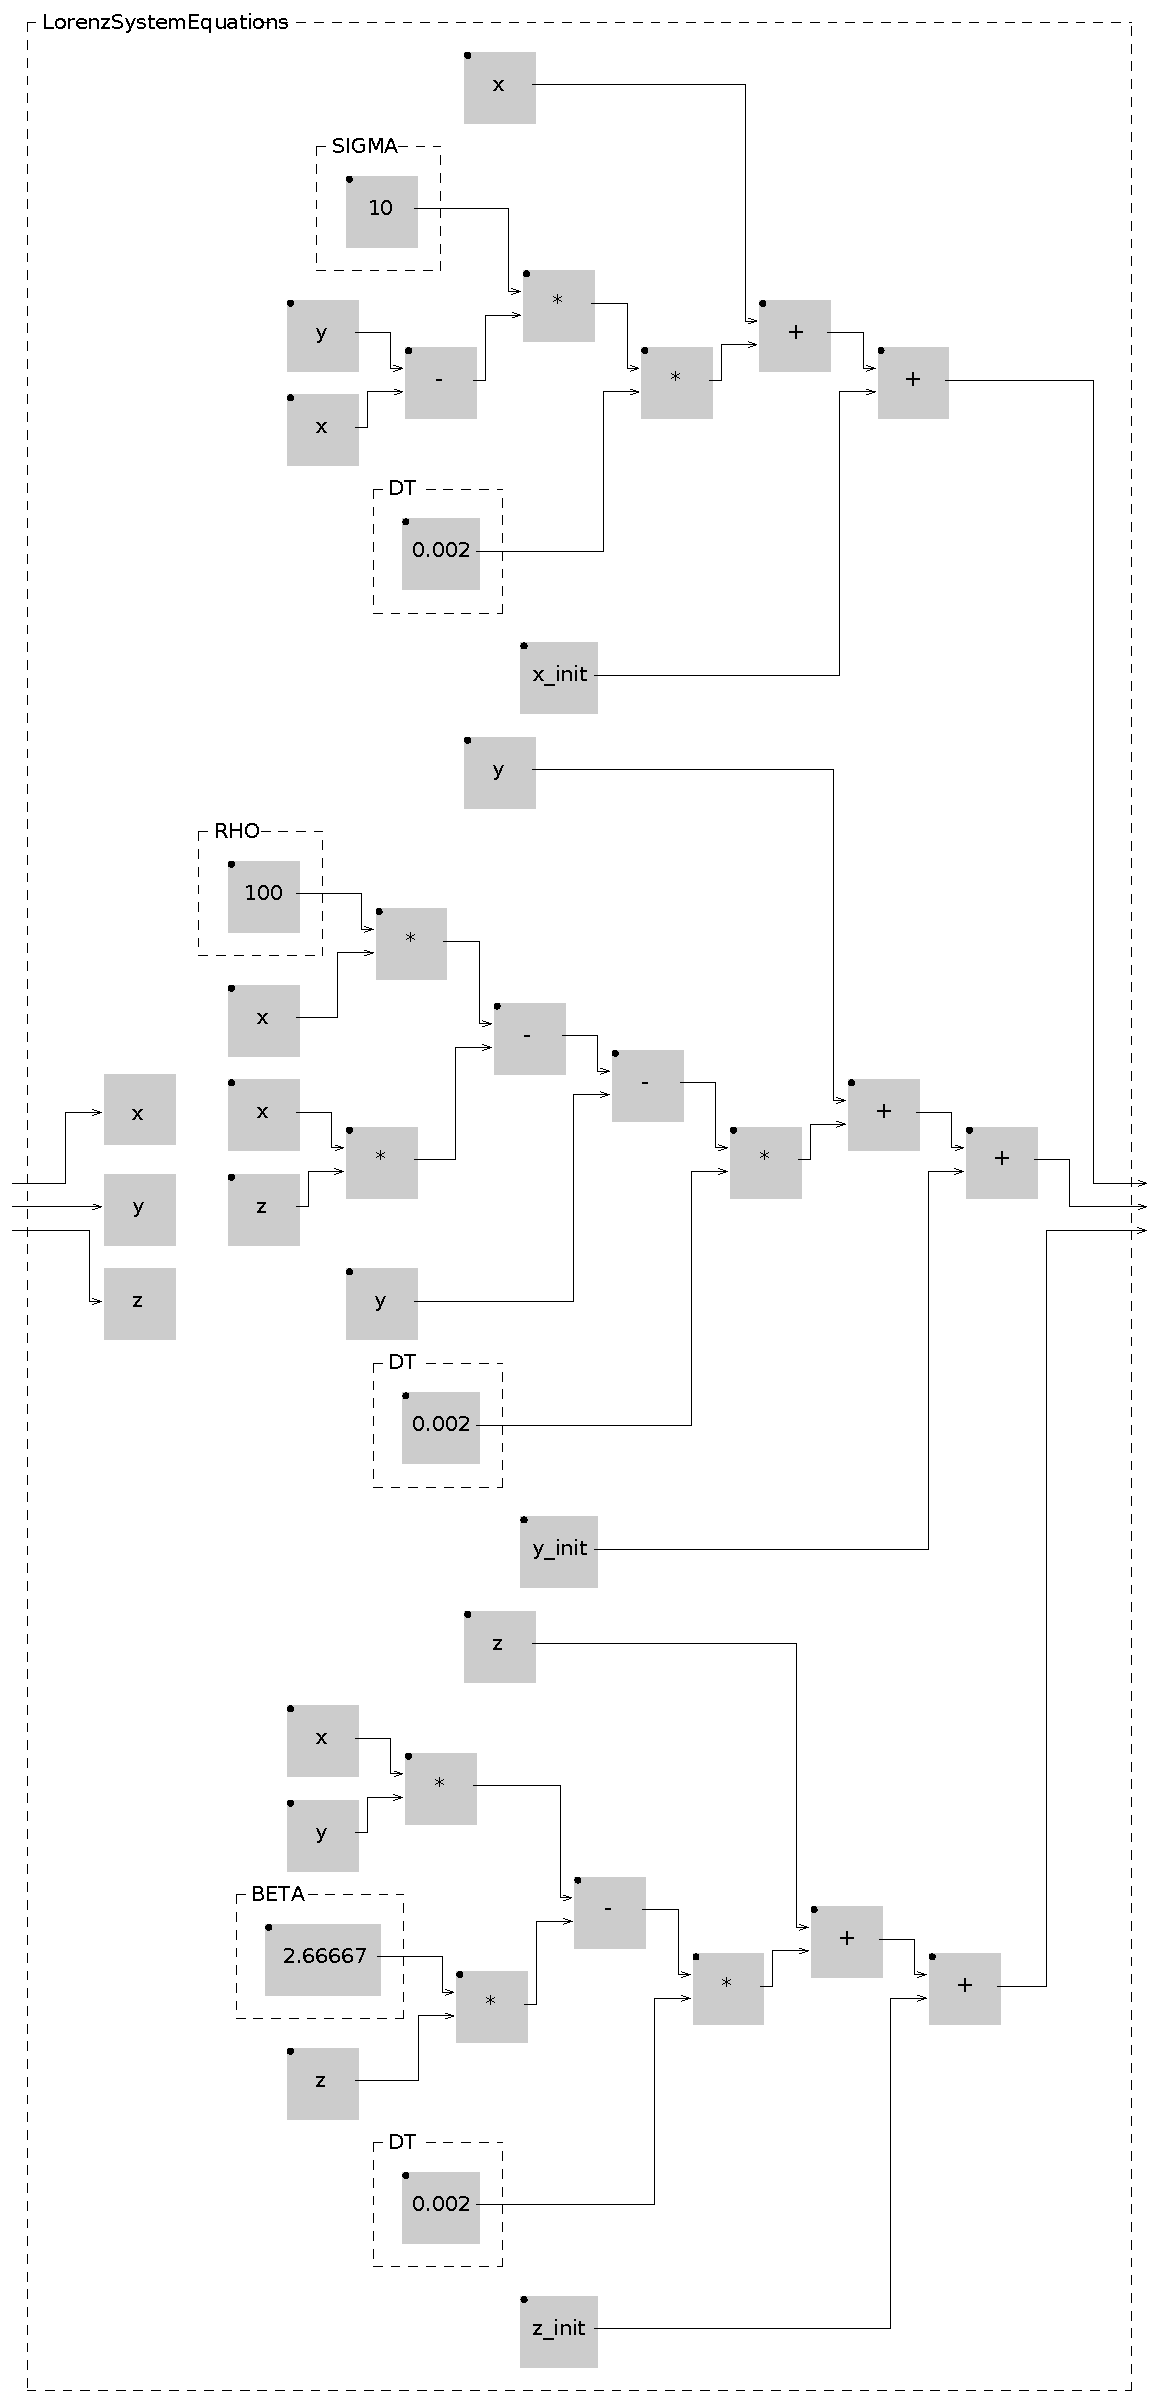
\includegraphics[width=11.5cm]{figures/LorenzSystemInside.pdf} 
    \caption{Topologia dell'Algoritmo del Sistema di Lorenz Discreto} 
\end{center}
\vspace{0.5cm}
\end{figure}
\clearpage

\begin{figure}[h!]
\begin{center}
    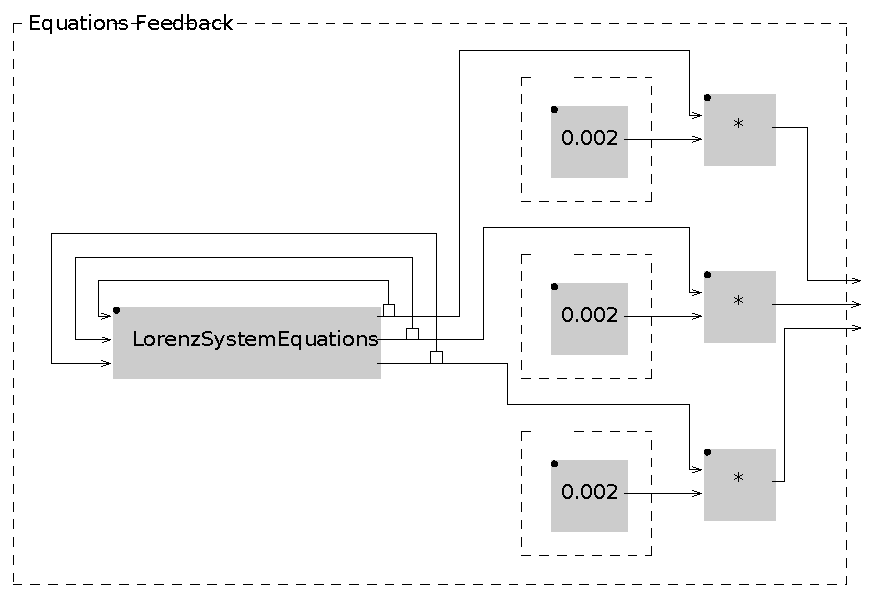
\includegraphics[width=14cm]{figures/LorenzSystemFB1.pdf}
    \caption{Topologia del Feedback delle Equazioni del Sistema di Lorenz Discreto}
\end{center}
\vspace{0.5cm}
\end{figure}

Questo algoritmo permette già di produrre sintesi attraverso la 
risoluzioni delle Equazioni del Sistema di Lorenz, ma per il momento in modo acritico.
Come detto in precedenza, esistono ricerche che si pongono il problema 
di un adattività dei sistemi caotici con il fine di poterli utilizzare per determinati scopi,
andrò adesso ad illustrare nel dettaglio i modelli che ho preso 
a riferimento in questo brano per poter utilizzare
i sistemi caotici per fini musicali di sintesi del segnale. \\
Per poter esplorare un sistema caotico con il fine di creare un segnale udibile in tutte le sue regioni, 
è necessario dunque porsi dunque un problema di ottimizzazione;
è necessario chiedersi quali problemi possano verficarsi e quali strumenti possano contrastarli. 
I problemi nell'utilizzare Lorenz come segnale di sintesi 
sono in sostanza Il DC Offset, e i valori più grandi del range [1, -1].
Riguardo le soluzioni sappiamo che il DC blocker, 
è uno strumento indispensabile nella modellazione della guida d’onda
digitale e in altre applicazioni, e che può rimuovere la componente Continua del segnale 
che circola in una linea di ritardo. Questo consiste sostanzialmente in
un filtro FIR highpass, poiché le correnti continue possono essere viste come frequenze a
0Hz, ed infine un onepole in serie che recupera parte della cancellazione del FIR.
Mentre per la funzione della tangente iperbolica, sappiamo che è una funzione
non lineare appartenente alle funzioni iperboliche, che costituiscono una famiglia di funzioni 
elementari dotate di alcune proprietà analoghe e corrispondenti alle
proprietà delle ordinarie funzioni trigonometriche.
utilizzando la tangente iperbolica come un Waveshaper (soft clipping) possiamo 
esplorare il sistema caotico in tutte le sue regioni rimanendo sempre in un range [1, -1].
A tal proposito Dario Sanfilippo propone:\footcite{sanfilippo_constrained_2021}

\begin{quote}
    Considering first-order differential equations, 
    we can obtain a generalisation of the modified systems discussed
    here. Let \( y \) be a vector of functions, let \( x \) be an input vec-
    tor, let \( F \) be a vector of functions of \( y \) and \( x \) ; let  \( C \) be
    a vector of constraining functions. Written in differential
    form with respect to time, we have that:
\end{quote}
\begin{center}
\begin{align*}
    \frac{\partial y(t)}{\partial t} & = C(F(x(t), y(t))) && \text{where} && C(z) = B(l * S(z(l)))
\end{align*}
\end{center}
\begin{quote}
    with B and S being, respectively, vectors of first-order
    DC-blockers and saturating nonlinearities with arbitrary
    saturation threshold piloted by the parameter l. The saturation threshold 
    becomes a key parameter for the interaction with the oscillators, while the overall output can be
    normalised to unity peak amplitudes for digital audio by
    merely dividing by l. While several types of bounded saturators are available, here, 
    we will focus on the well known 
    hyperbolic tangent function. Note that the input
    vector can be used to set the system’s initial conditions or
    as continuous perturbation through signals. In fact, these
    systems can also be deployed as nonlinear distortion units
    when operating under non-self-oscillating conditions.
\end{quote}

Secondo il metodo appena esposto, le costrizioni possono essere rappresentate come

\begin{align*}
    \text{where B} && y(n) = x(n) -x(n-1) +Ry(n-1) \\
    \text{where S} && y(t) = tanh(x(t))
\end{align*}

Mentre per la rappresentazione di Lorenz in forma di modello discreto modificato,
può essere scritto un algoritmo in Faust come segue:

\vspace{0.5cm} 
\lstinputlisting[breaklines, frame=trBL, caption={Algoritmo del Sistema di Lorenz Modificato con DC-blocker e TanH}]
{codes/CostrainedLorenzSystem.dsp}

\begin{figure}[h!]
\begin{center}
    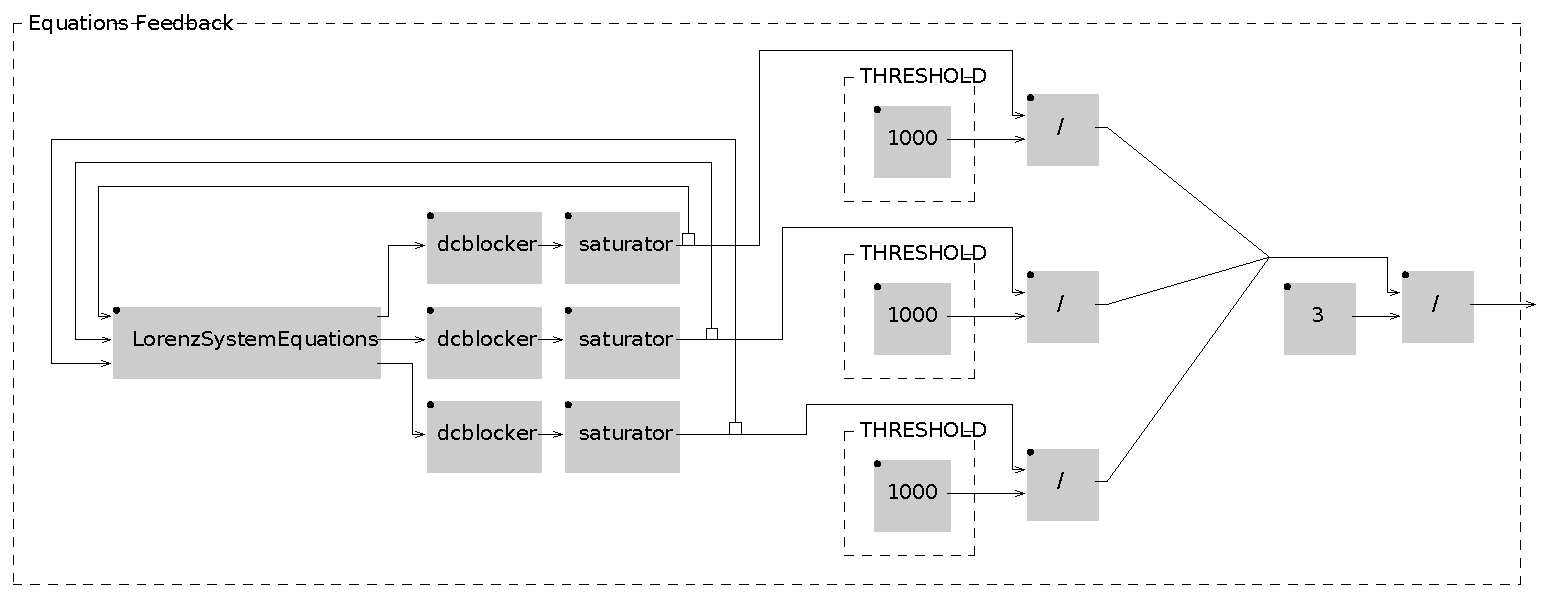
\includegraphics[width=14cm]{figures/LorenzSystemFB2.pdf}
    \caption{Topologia del feedback delle Equazioni del Sistema di Lorenz Modificato con DC-blocker e TanH}  
\end{center}
\vspace{0.5cm}
\end{figure}

\begin{figure}[h!] 
\begin{center}
    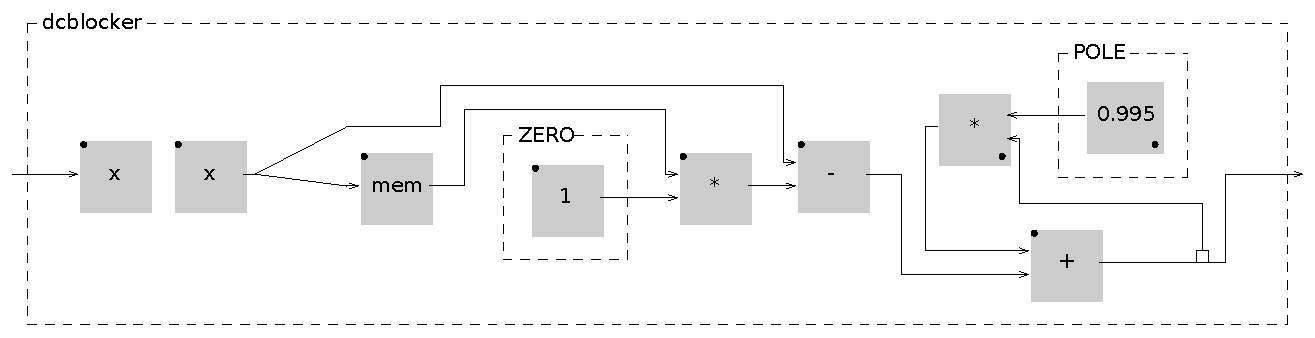
\includegraphics[width=14cm]{figures/DCblocker.pdf}
    \caption{Topologia dell'Algoritmo DC-blocker} 
\end{center}
\vspace{0.5cm}
\end{figure}
\clearpage

\begin{figure}[h!] 
\begin{center}
    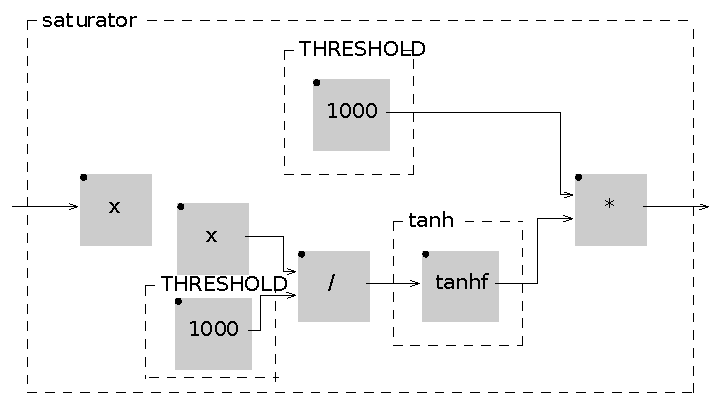
\includegraphics[width=10cm]{figures/Saturator.pdf}
    \caption{Topologia dell'Algoritmo TanH} 
\end{center}
\vspace{0.5cm}
\end{figure}

Ora il sistema di Lorenz è invece ottimizzato per la sintesi sonora.
Per concludere, il sistema di Lorenz Modificato passa infine per la sua terza costrizione,
che consiste in un Banco di Filtri Bandpass dove per un solo termine in ingresso 
il segnale viene diviso per il numero di banchi di filtri e restituito in uscita. \\
Il banco di filtri Bandpass è costituito da 32 voci parallele informate da 
4 liste di ricavate da analisi di 4 file audio di note del violocello,
esplorate durante il corso della performance.
L'algoritmo dei filtri Bandpass utilizzato come costrizione per il sistema
di Lorenz Modificato, consiste in un implementazione \textit{Virtual Analog} 
di un filtro del 2° ordine basato sulla struttura SVF \textit{State Variable Filter}.
La particolarità di questo tipo d'implementazione di SVF che ho utilizzato,
è che preserva matematicamente la topologia del filtro analogico,
includendo nella maggiorparte dei casi \textit{zero-delay loops}.
Questi filtri sono chiamati \textit{Topology Preserving Transform filters} o filtri TPT,
e provengono dal libro "The Art of VA Filter Design" di Vadim Zavalishin,\footcite{Zavalishin_VA_filter_design}
pubblicato e reperibile gratuitamente in rete. \\
A seguito riporto l'implementazione matematica di questo filtro SVF TPT di Vadim Zavalishin
che ha esposto Will Pirkle in un suo articolo chiamato 
"Virtual Analog (VA) Filter Implementation and Comparisons v2.0"\footcite{Pirkle_VA_filter_design}
del 2013 e reperibile dal suo sito.

\begin{align*}
    y_{hp}(n) = & \frac{x(n)- 2Rs_{1}(n) - gs_{1}(n) - s_{2}(n)}
    {1 + 2Rg + g^{2}}
\end{align*}

in questa formula viene prima calcolata l'equazione 
differenziale per l'uscita \( yHP \) (Highpass),
e dopo, applicata all'ingresso del primo integratore, 
utilizzando il metodo il \textit{read-before-write}
(ovvero \( s_{1} \) e \( s_{2} \) vengono letti per primi e aggiornati per ultimi). 
Vengono ricavate da qui le equazioni alle differenze per tutti gli altri filtri:

\begin{align*}
{y_{bp}(n)}& =  gy_{hp}(n) + s_{1}(n) \\
{y_{lp}(n)}& =  gy_{bp}(n) + s_{2}(n) \\
{y_{ubp}(n)}& =  2Ry_{bp}(n) \\
{y_{bshelf}(n)}& =  x(n) + 2KRy_{bp}(n) \\
{y_{notch}(n)}& =  x(n) - 2Ry_{bp}(n) \\
{y_{apf}(n)}& =  x(n) - 4Ry_{bp}n) \\
{y_{peak}(n)}& =  y_{lp}(n) - y_{hp}(n) \\
\end{align*}

prendendo quindi la funzione \( y_{bp} \), e assumendo ancora una volta C come vettore delle costrizioni
per le tre equazioni differenziali del sistema di Lorenz, 
e aggiungendo ora Q come la funzione che rappresenta il banco di filtri, 
avremo infine che:

\begin{gather*}
    \text{for} \frac{\partial y(t)}{\partial t} = C(F(x(t), y(t))) \\
    \text{where} C(z) = Q(B(l * S(z(l)))) \\
    \text{Q is} y(n) = x_{1bp}(n) + x_{2bp}(n) + x_{3bp}(n) + ... x_{32bp}(n)
\end{gather*}

il CSGA in forma di modello discreto modificato,
può infine essere scritto in un algoritmo in Faust come segue:

\vspace{0.5cm} 
\lstinputlisting[breaklines, frame=trBL, caption={Algoritmo del Sistema di Lorenz Modificato con Filterbak}]
{codes/CSGA.dsp}

\begin{figure}[h!]
\begin{center}
    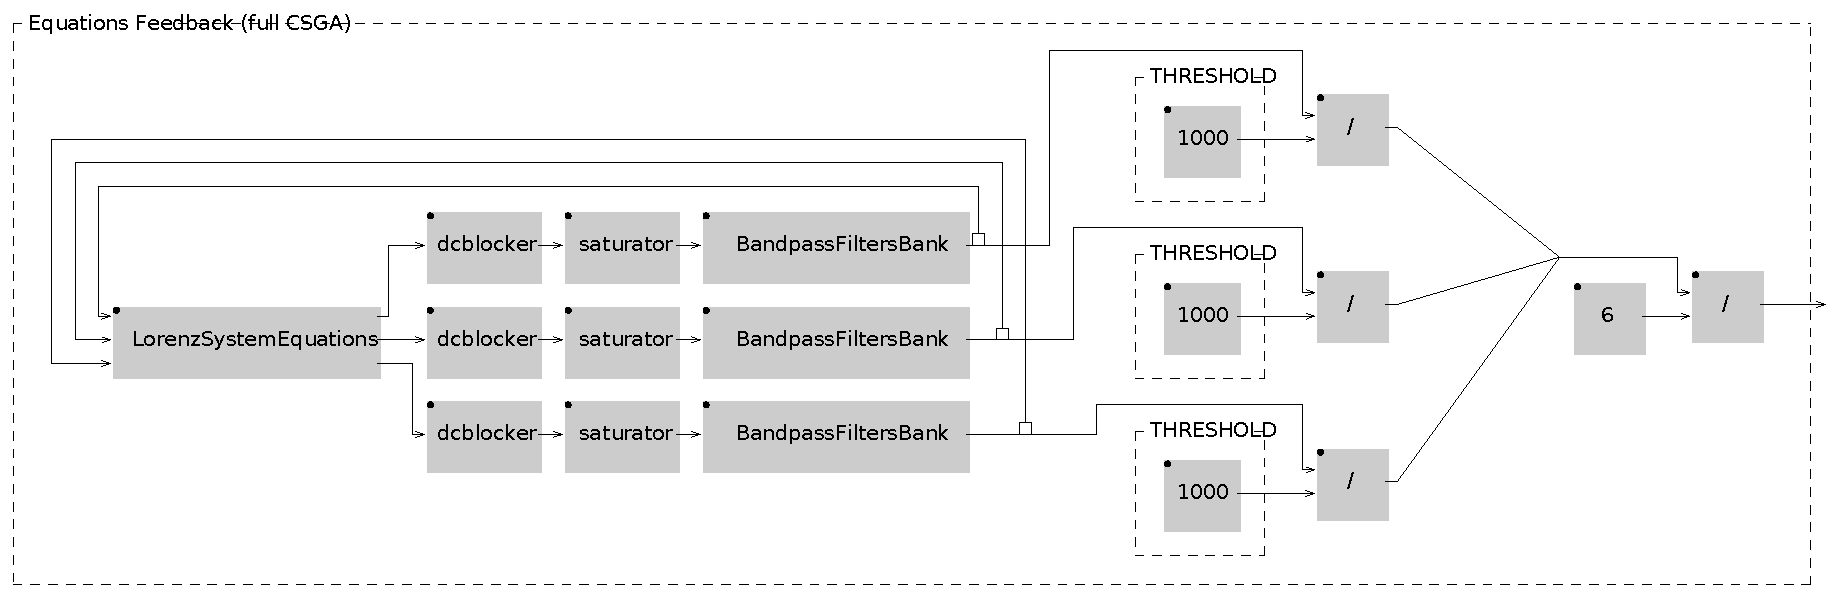
\includegraphics[width=14cm]{figures/LorenzSystemFB3.pdf}
    \caption {Topologia del feedback delle Equazioni del Sistema di Lorenz Modificato con Filterbank}
\end{center}
\vspace{0.5cm}
\end{figure}

\clearpage
\begin{figure}[h!]
\begin{center}
    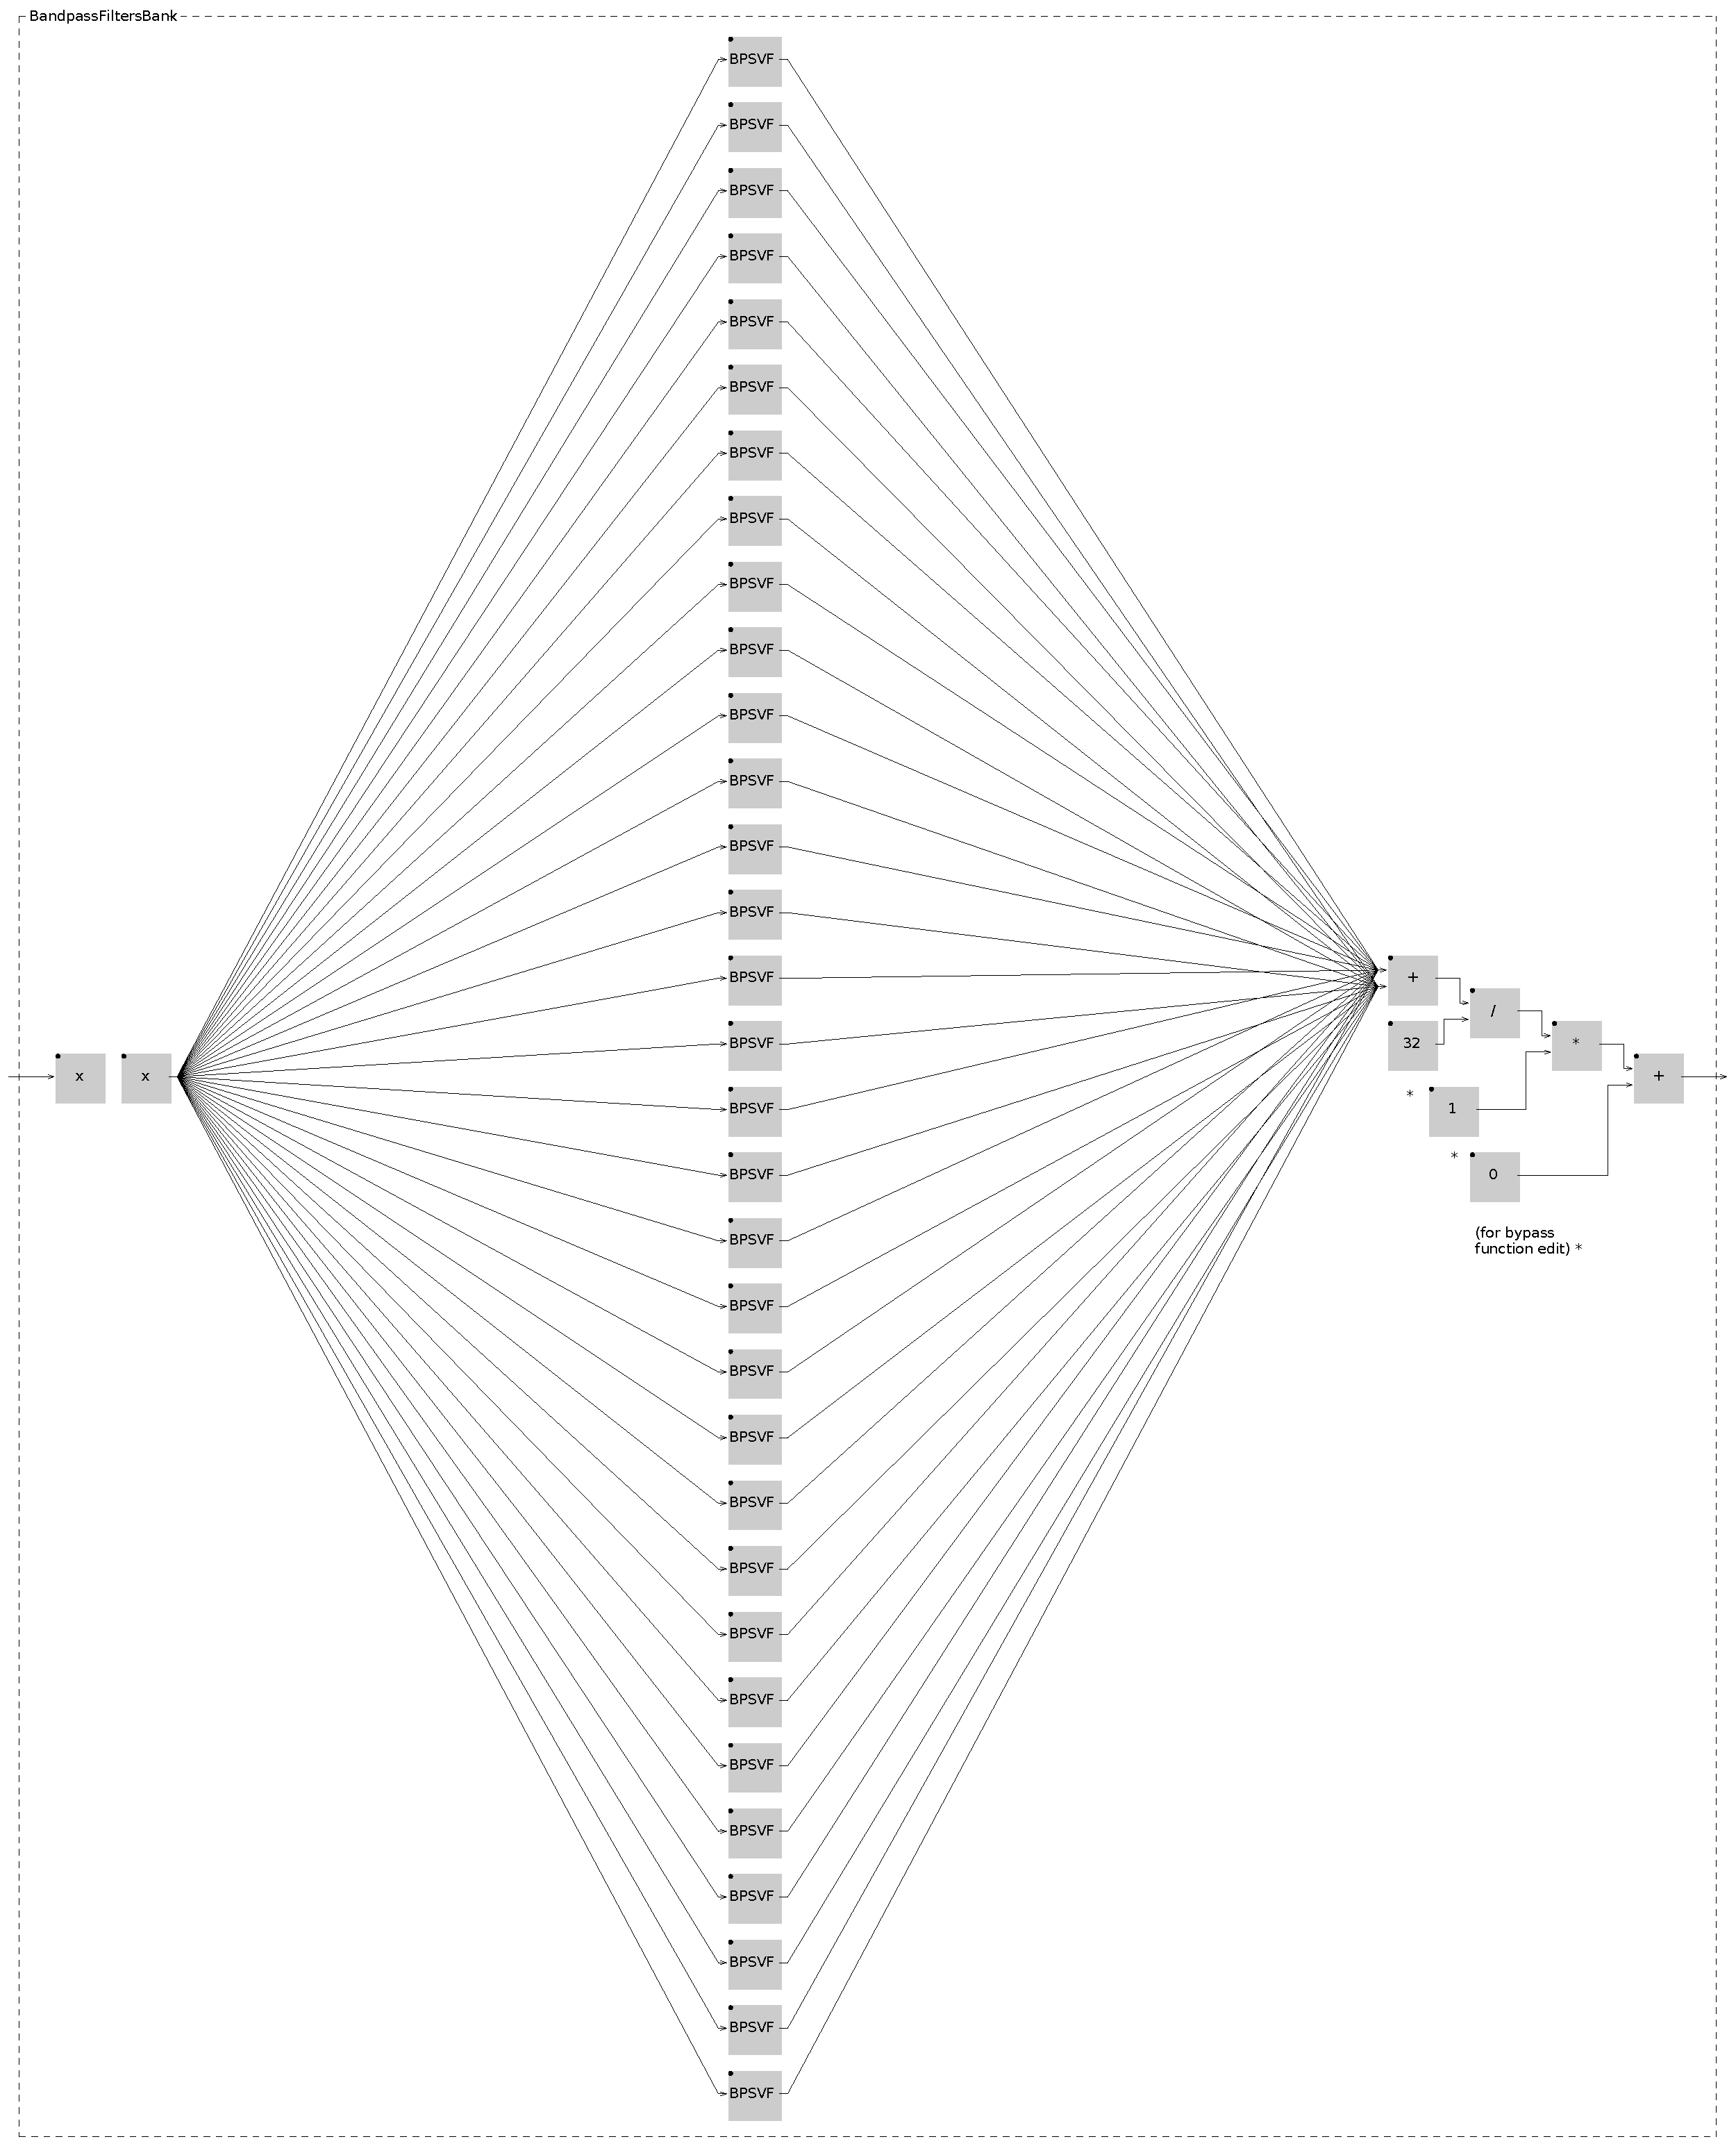
\includegraphics[width=15cm]{figures/BPFilterBank.pdf}
    \caption{Topologia del Filterbank con i filtri Bandpass SVF TPT}
\end{center}
\vspace{0.5cm}
\end{figure}

Questo andrà a rappresentare un singolo Agente richiamato all'interno della FDN.
Prima di passare alla descrizione globale della rete,
voglio ringraziare qui Edoardo Staffa per avermi assistito 
nel realizzare un semplice metodo di analisi DFT per i file audio .wav 
tramite alcune librerie nel Linguaggio di programmazione Python3.
In un secondo momento ho poi modificato il codice per 
ottenere le liste con il metodo che mi occorreva per informare i filtri di Faust.
Gli algoritmi in Python3 utilizzati per le Analisi dei file audio si trovano nel
secondo appendice.

\subsection{Feedback Networks}
\label{Feedback Networks}

Per concludere questa osservazione sulla struttura sistemica di RITI,
discuterò brevemente, ripetendo alcuni concetti fondamentali illustrati ad inzio capitolo.
I tre stati di feedback principale su cui si basa questo sistema sono:
Il feedback interno alle equazioni differenziali, o chiamato anche come fattore di magnificazione; 
ne possiamo vedere un implementazione in questo paper\footcite{liang_difference_2013}.
Questo ci permette di poter portare le equazioni di Lorenz da uno stato di autoscillazione al
solo funzionamento come funzione di trasferimento (waveshaping) per il segnale in ingresso.
Il feedback della FDN, permette ai segnali presenti nella rete di ricircolare
con opportuni tempi di ritardo, così da avere delle decorrelazioni fra i CSGA, oltre che dei comportamenti del sistema
che possano avere una loro storia nel tempo, anche nel tornare quando il fattore di magnificazione di Lorenz è pari a 0
così da poter apprezzare solo la storia del sistema all'interno della rete senza avere nuovi contributi.
Ed infine, poiché ho dotato le equazioni di Lorenz di un ingresso esterno che viene sfruttato
sia dalla reiniezione dei segnali provenienti dalla FDN, che dall'aggiunta di 4 microfoni esterni,
il sistema viene aperto all'ambiente: perturbato dagli stessi segnali che produce all'interno della stanza,
che ne variano il comportamento nel tempo, e da fenomeni di Larsen che emergono quando il fattore di 
magnificazione che produce l'autoscillazione in Lorenz ha un contributo energeticamente 
inferiore rispetto a quello del Larsen proveniente dalla stanza.
\clearpage

\begin{figure}[h!]
\begin{center}
    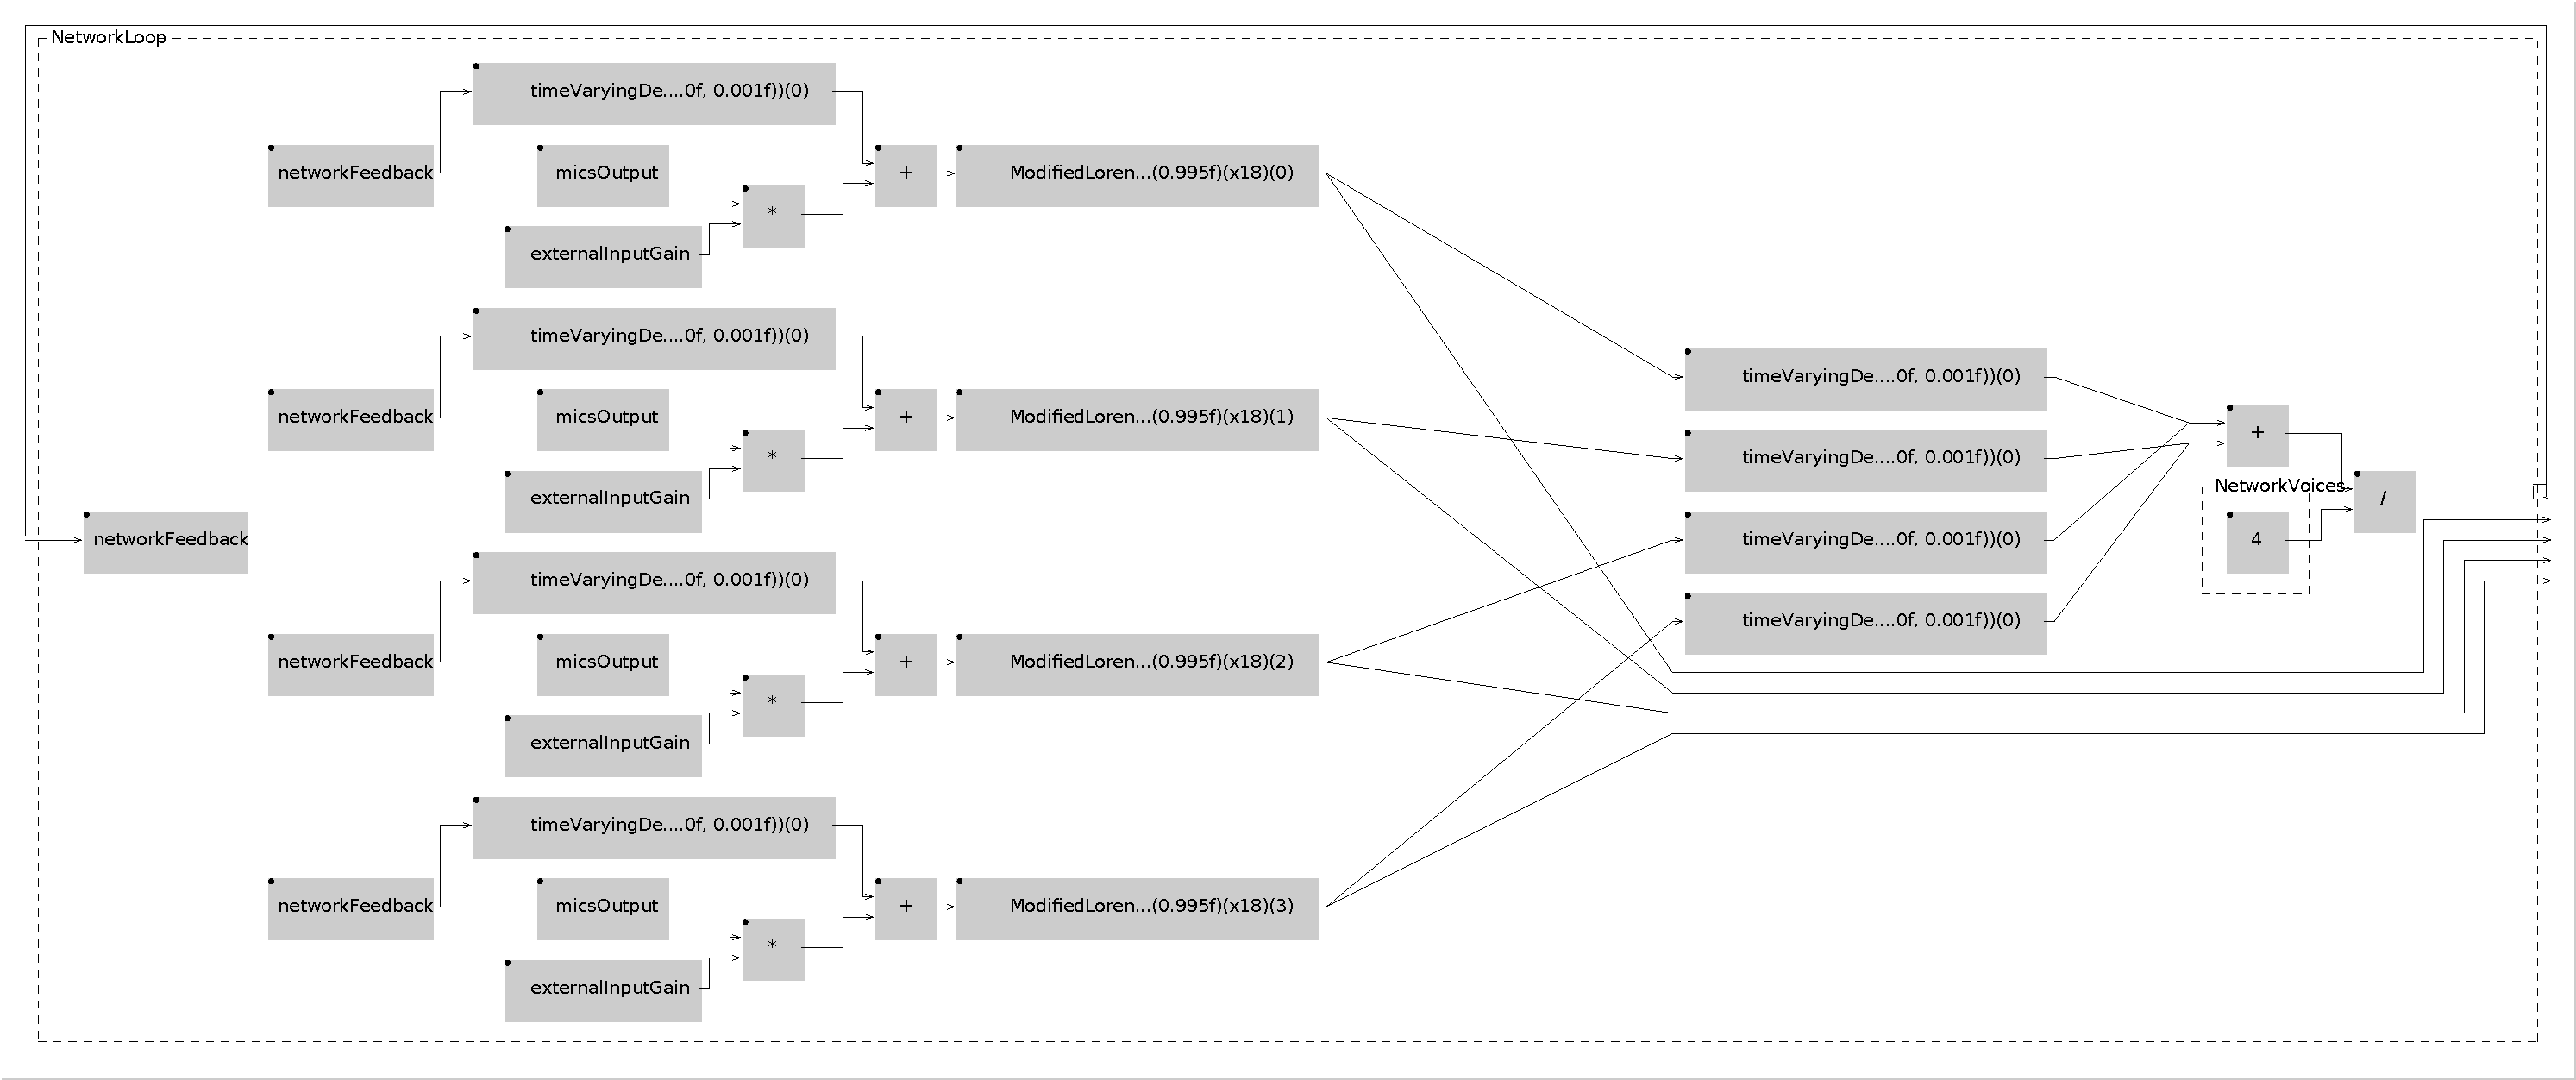
\includegraphics[width=15cm]{figures/RITI4VoiceNetwork.pdf} \\
    \caption {Esempio della Rete di RITI compilata con 4 Voci (4 CSGA)}
\end{center}
\end{figure}

\vspace{0.5cm}

La possibilità di regolare i tre stati di feedback e di portare il sistema "sulla soglia del caos"
esplorando nella performance tutti i suoi spazi, 
rivolgendo gli altoparlanti verso le pareti trasformando così l'ambiente stesso
nello spazio di sistema, rappresenta per me un estensione: del concetto di strumento musicale, 
dell'interazione con la macchina, ed infine dell'utopia di un nuovo ascolto,
in un mondo dove è sempre più necessario prendere consapevolezza della complessità che ci circonda.

\subsection{Motivazioni Personali}
\label{Motivazioni Personali}

Prima di concludere questo elaborato, 
vorrei prima soffermarmi a spiegare alcune delle motivazioni 
personali che hanno suscitato in me l'interesse per i 
sistemi complessi adattivi in live electronics, 
e che mi hanno spinto in particolare alla creazione di questo brano. \\
In questi ultimi anni di studi musicali, sono emerse nel mio fare musica 
delle questioni per me di fondamentale importanza che hanno accompagnato il mio operato
e che hanno mosso il mio interesse verso i le cibernetiche in musica. \\
In primo luogo indagare rispetto al rapporto che esiste fra l'interprete, la notazione, e lo strumento musicale;
che può essere vista in qualche modo come una parte contenuta all'interno 
della relazione fra uomo-macchina-ambiente di cui parla
Agostino Di Scipio. \\
Le prime forme di semiografia musicale possono essere rintracciate in diverse civiltà 
che risalgono addirittura attorno al 2000 A.C.,
sin d'allora l'uomo ha posto al centro della sua indagine l'interrogativo sul come fissare sempre meglio 
successioni strutturate di suoni semplici o complessi tramite una serie di parametri nel dominio discreto (la notazione), 
e che interpretati in un secondo momento potessero restituire l'idea iniziale in una resa 
acustica nel dominio del continuum temporale.
Questi parametri principalmente impiegati nella semiografia musicale Occidentale, 
sono stati fino all'incirca ad inizio del XX Secolo: 
le altezze dei suoni, le intensità, i ritmi, le durate, ed infine il timbro desiderato, 
quest'ultimo descritto richiedendo l'impiego di un certo strumento musicale o di specifici gruppi strumentali.
Tuttavia il significato stesso del termine musica non è comunque univoco ed ha avuto (ed ha ancora ad oggi) 
diverse accezioni utilizzate nei vari periodi storici.
Difatti con l'arrivo del XXI Secolo, sono state messe in crisi le nozioni di strumento musicale e di semiografia musicale, 
in quanto la pratica del comporre non si è più solamente limitata al comporre 
con i timbri dei diversi strumenti musicali, ma si è aperta anche alla possibilità del comporre stesso nel timbro, 
spingendo i compositori a cercare vie alternative ed alle volte individuali in cui scrivere musica differente dalla tradizione.\\
Riguardo gli strumenti musicali invece, se la voce è difatti il primo strumento dell'uomo in quanto 
abita il corpo stesso che ne è il custode, la macchina che nel suo senso generico è qualsiasi strumento 
il cui moto relativo trasmetta o anche amplifichi la forza umana.
Sin dall'antichità la macchina si è prestata all'impiego come strumento musicale sottoforma di qualcosa per assistere l'uomo nella 
sua intenzione del fare musica secondo l'organizzazione dei parametri esposti precedentemente; 
con la composizione nel timbro viene invece a mancare l'idea 
di una musica composta solamente da queste tipiche relazioni tramite gli strumenti musicali, 
rivalutando l'idea stessa che si ha di uno strumento musicale, aperta ora di fatto alla possibilità 
del poter comporre quanto il timbro stesso integrando anche la creazione dello strumento che lo produce. \\
Come dice Trevor Wishart nel suo libro On Sonic Art:

\begin{quote}
    In this book i will suggest that the logic of this assertion is inverted.
    It is notability which determines the importances of pitch, rythm, and duration and
    not vice versa and that much can be learned by looking at 
    musical cultures without a system of notation... 
    In this book, I will suggest that we do not need to deal with a finite set of
    possibilities. The idea that music has to be built upon  finite lattice and the
    related idea that permutational procedures are a valid way to proceed will
    be criticised here and a musical methodology developed for dealing with a
    continuum using the concept of transformation \footcite{wishart_on_sonic_art}
\end{quote}

Come comportarsi quindi davanti ad una condizione in cui viene messa in crisi l'idea stessa
che si ha di musica, di notazione musicale, e di strumento musicale?\\
Questa indagine mi ha portato a rivolgere l'attenzione al rapporto con la notazione 
e gli strumenti musicali in quelle opere dei compositori contemporanei, 
che raccogliendo le ceneri di questa crisi del XXI Secolo, 
hanno deciso di approfondire l'idea dietro l'utilizzo
di uno strumento musicale con cui fare musica, non più come 
qualcosa di funzionale al riprodurre dei parametri annotati in partitura a priori,
ma come un sistema che offre una serie di possibilità; 
in cui lo strumento diviene il corpo acustico su cui indagare 
tutta una serie di relazioni e gesti possibili dell'interprete, 
alla ricerca di un'esplorazione sonora dello spazio del sistema,
e in cui la partitura diviene traccia del come replicare l'esistenza di 
qualsiasi tipo d'interazione con il sistema.
In tal senso Trevor Wishart suggerisce di guardare alla Teoria delle Catastrofi 
di René Thom, assumendo che le regole formali di una musica passono
essere ricavate dall'osservazione di uno strumento stesso come se questo fosse un sistema.
Nella mia indagine per portare dei validi esempi, ho dunque rintracciato questo tipo di atteggiamento 
nei confronti dello strumento
e della notazione in alcune opere come: Pression di Helmut Lachenmann,
dove la partitura viene ad indicare come agire sul corpo dello strumento
schiudendone nella sua totalità il suo mondo sonoro accessibile,
o nell'opera Necessità d'interrogare il cielo di Giorgio Netti,
dove a partire dagli elementi della notazione tradizionale, lo studio condotto 
sul corpo dello strumento e degli esiti acustici del gesto, scendono così tanto 
"ad un basso livello di articolazione" da schiuderne in questo tutta una serie di nuove possibilità
acustiche, o anche nei lavori stessi di Wishart, come nel ciclo Vox 
dove la voce viene esplorata in tutte le sue ambiguità rendendo
complesso il collegamento fra il suono e la sorgente che lo produce. \\
In senso più generale la storia della musica elettroacustica è fortunatamente costellata 
di pionieri che hanno messo in crisi il linguaggio musicale e l'impiego degli strumenti musicali,
ma l'ulteriore scarto che propongo qui, consiste nel fatto che se è vero quindi come 
dice Trevor Wishart che le regole formali di una musica possono
essere ricavate dall'osservazione di un sistema, 
la pratica del disegnare un sistema autonomo (la macchina) con cui fare musica,
ne riflette di conseguenza la quantità di informazione che questo contiene al suo interno,
e di conseguenza il tipo di relazioni e interazioni con il suo ambiente che 
ci interessano dal punto di vista compositivo.\\
In secondo luogo, ho trovato interessante indagare rispetto al rapporto conflittuale che l'uomo ha con la tecnologia
nella società contemporanea. 
In effetti, l'uomo ha da sempre un rapporto conflittuale con la tecnologia,
se sin dai tempi di Platone emergevano queste problematiche e preoccupazioni
relative alla discretizzazione del pensiero con la scrittura
(come possiamo leggere in Fedro), 
giungendo alle paure più attuali di Norbert Weiner di fronte
alla scoperta della cibernetica, possiamo dire che la sua paura di una società contemporanea 
composta da interazioni sistemiche fra l'uomo e la macchina
in cui il primo è succube della seconda, sembra in qualche modo essere stata profetica ed essersi realizzata.
Come scrive Norbert Wiener nel suo libro Introduzione alla cibernetica. L'uso umano degli esseri umani,
inizialmente pubblicato con il titolo The Human Use Of Human Beings: Cybernetics And Society \footcite{wiener_introduzione_nodate}
nel 1950:

\begin{quote}
    La nostra concezione della società ideale differisce dalla società ideale
    prospettata dai fascisti e da molti magnati del mondo degli affari 
    e della politica.
    Essi preferiscono una organizzazione in cui tutti i comandi
    provengano dall'alto senza che sia possibile nessuna riverisbilità.
    Sotto di essi gli uomini sono stati ridotti al livello di esecutori degli ordini
    di un centro nervoso che pretende di essere superiore.
    Desidero che questo libro sia inteso come una protesta contro questa
    utilizzazione inumana degli esseri umani, poiché sono convinto che impiegare
    un uomo richiedendogli e attribuendogli meno di quanto comporta la sua condizione umana,
    significa abbruttire questa condizione e sperperare le sue energie.
    È una degradazione della condizione umana legare un uomo a un remo e impiegarlo come
    sorgente di energia; ma è altrettanto degradante segregarlo in una fabbrica
    e assegnarlo a un compito meramente meccanico che richieda meno di un milionesimo
    delle sue facoltà cerebrali. È assai più facile infatti
    organizzare una fabbrica o una galera che impieghi gli esseri umani
    per una insignificante frazione delle loro attitudini che costruire una 
    società in cui essi possano elevarsi in tutta la loro statura.
    Coloro che soffrono di un complesso di potenza sanno che la meccanizzazione 
    dell'uomo è il mezzo più semplice per realizzare le loro ambizioni.
    Sono convinto che questa facile via al potere comporta non soltato l'annullamento 
    di quelli che io credo siano i valori morali dell'umanità,
    ma anche l'eliminazione delle attuali, labilissime possibilità di
    sopravvivenza della razza umana per un periodo considerevole.
\end{quote}

Se in risposta a questa affermazione di Wiener passiamo ad una seconda citazione, proveniente invece da un libro 
recente che critica la nostra condizione nella società contemporanea, scritto e pubblicato da François J. Bonnet. nel 2020:

\begin{quote}
    The increasingly frenetic accumulation of sounds and
    images is a part of this intensification, aiming to fill the void of
    a present that is forever sinking into the past. At every
    moment, the world must be supplied with novel sensory
    material generated to replace existing material that has
    already become obsolete. The exaltation of the present as the
    promise of pleasure Is therefore never really meant to be actualised,
    since it will immediately be obsolesced by a continuously
    renewed influx of promises.
    Needs, cravings, and desires
    are endlessly rebooted.
    The present moment, as constructed by our society, is
    nothing but a procedure of forgetting, a catalyst for amnesia,
    and as such it enables the repetition which, in turn, through
    the presentation of novelty, allows us to distance ourselves
    3 little further from the past. And this writing and rewriting
    of the present—as if it were a palimpsest—continues to
    accelerate, demanding that we forget at an ever higher fre-
    quency. What was is of no concern; all has beens are eliminated
    in favour of what is, with little regard for what will be.
    Where the modern era anticipated a present yet to come,
    transposing current momentum into future accomplishments,
    our postindustrial, postmodern era sees the future as
    nothing but a vague, indeterminate site hosting an indistinct
    cloud of promises and signs as desirable as they are deadly. \footcite{francois_jbonnet_after_death}
\end{quote}

Troveremo che non solo le paure profetiche di Wiener si sono realizzate già da diverso tempo, 
ma che da molto tempo ne stiamo già raccogliendo le inevitabili conseguenze,
che si riflettono dal mio punto di vista in una società anestetizzata, 
schiava della tecnologia, e livellata in qualche modo ad una condizione di eterno presente.
In risposta a questa condizione, disegnare i propri sistemi e di conseguenza riappropriarsi della tecnologia,
rappresenta per me un modo costruttivista di rispondere ai problemi del mondo contemporaneo
attraverso la pratica musicale.\\
Per concludere infine le motivazioni che mi hanno portato a questo tipo di scrittura musicale, 
l'ultimo aspetto che ho reputato importante affrontare è la forma,
nei suoi aspetti Macro-temporali e Micro-temporali. \\
Se ammettiamo quindi come sostiene François J. Bonnet, ed altri filosofi come Mark Fisher e Slavoj Žižek,
che la nostra società contemporanea ha in qualche modo normalizzato
una velocità schizofrenica nelle cose, dove tutto deve essere estremamente funzionale per motivi pratici,
e dove non abbiamo più modo di esercitare alcun controllo sullo scorrere del tempo,
la riappropriazione del tempo nella forma, dell'ascolto, ed infine dello spazio, diviene per me un elemento fondamentale
nella composizione,
dove tutti gli elementi del sistema hanno un ruolo condiviso che contribuisce 
a formare la complessità nel suo insieme.
A tal proposito ho sempre trovato interessante osservare nelle evoluzioni temporali 
come un piccolo cambiamento all'interno di un sistema possa conseguentemente portare 
a cambiamenti radicali
nella Macroforma; proprio come nella sensibilità alle condizioni della teoria del caos, 
che ci illustra come in un sistema caotico, a variazioni infinitesime delle condizioni iniziali 
corrispondono variazioni significative del comportamento futuro. 
Dunque in tal senso è diventato per me un aspetto importante lavorare con
sistemi emergenti che possano rendere udibili questi processi di continua trasformazione
del suono, e che non rendano udibile una sola traiettoria possibile nell'evoluzione formale
di un brano.\\
È a tal proposito che Stockhausen, nella sua teoria della "Forma unificata del tempo", 
notò già nel 1960 come in tal senso la differenza fra i Micro-elementi nella forma, 
e la Macroforma, non consista tanto in diversi ruoli e compiti del comporre,
quanto più a diversi livelli di percezione del tempo, 
poiché altezza e ritmo sono fondamentalmente la stessa cosa se percepita a diverse scale temporali,
e ce lo illustra nella sua composizione Kontakte realizzata fra il 1958 ed il 1960, 
mettendo in certi termini in luce,
come nella forma di un brano musicale il ruolo delle parti sia sostanzialmente un problema 
di complessità
che dipende dal punto di vista dell'osservatore.

%\subsection{Conclusioni}
%\label{Conclusioni}
%
%In conclusione, 
%abbiamo avuto modo di introdurre l'argomento delle cibernetiche in Musica,
%parlando di come l'esigenza di un pensiero sistemico 
%abbia pian piano fatto breccia nell'operato
%di alcuni dei più importanti compositori del XX Secolo. 
%Arrivando fino ad osservare e studiare il realizzarsi di questa condizione
%attraverso l'operato di Dario Sanfilippo e da Agostino Di Scipio, 
%di cui abbiamo approfondito alcuni dei principali meccanismi presenti nei loro lavori compositivi,
%nel desiderio di creare attraverso questi modelli
%una strada da seguire per la composizione dei sistemi complessi adattivi per la
%performance musicale in live electronics.
%Ed Infine mettendo in luce l'importanza di una prospettiva 
%ontologica ed epistemeologica nella composizione musicale sistemica.